

\begin{frame}{Ordered probit model}
  \begin{itemize}
    \item Model used for ordered but not interval or ratio scaled data
    \item Like linear regression, but with thresholds for the different categories
  \end{itemize}
\end{frame}

\begin{frame}{Ordered probit: example}
  \centering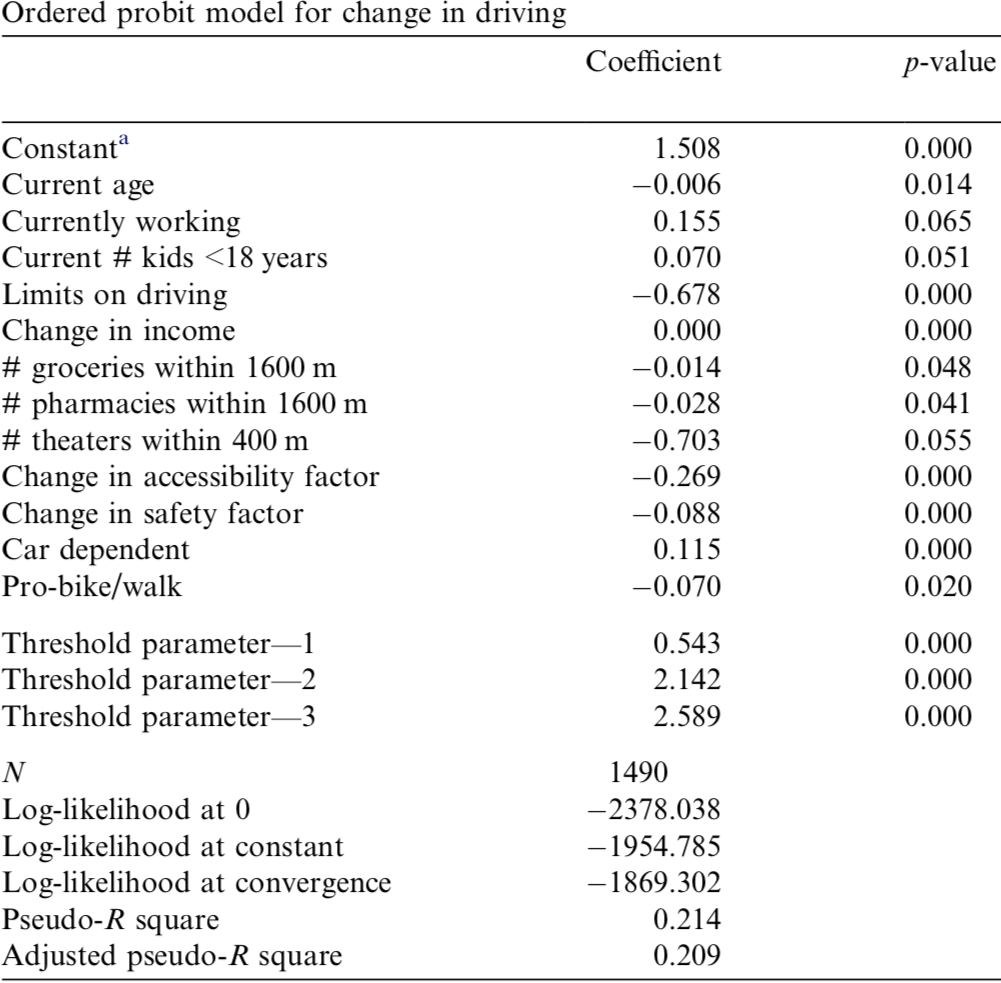
\includegraphics[width=0.5\textwidth]{img/handy_oprobit.png}\\
  \tiny \textcite{handy_correlation_2005}
\end{frame}

\begin{frame}{Ordered probit: example}
  \begin{equation*}
    y^* = 1.51 - 0.006 x_{\mathrm{age}} + 0.16 x_{\mathrm{working}} + 0.07 x_{\mathrm{children}} - 0.68 x_{\mathrm{limits on driving}} \cdots + \epsilon
  \end{equation*}

  \only<2>{\begin{equation*}
    y = \begin{cases}
      \text{a lot less now} & \text{if}~y^* \leq 0 \\
      \text{a little less now} & \text{if}~0 < y^* \leq 0.54 \\
      \text{about the same} & \text{if}~0.54 < y^* \leq 2.14 \\
      \text{a little more now} & \text{if}~2.14 < y^* \leq 2.59 \\
      \text{a lot more now} & \text{if}~2.59 < y^*
    \end{cases}
  \end{equation*}}

  {\tiny Based on \textcite{handy_correlation_2005}}
\end{frame}

\begin{frame}{Ordered probit: example}
  \only<1>{\centering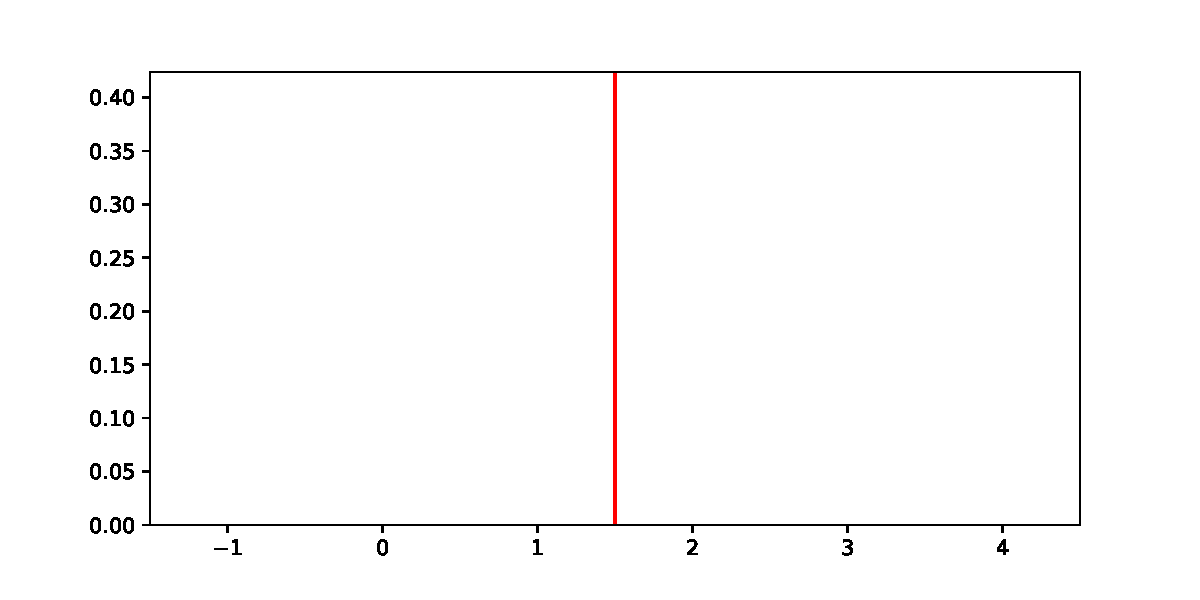
\includegraphics[width=\textwidth]{fig/oprobit_ystar.pdf}}
  \only<2>{\centering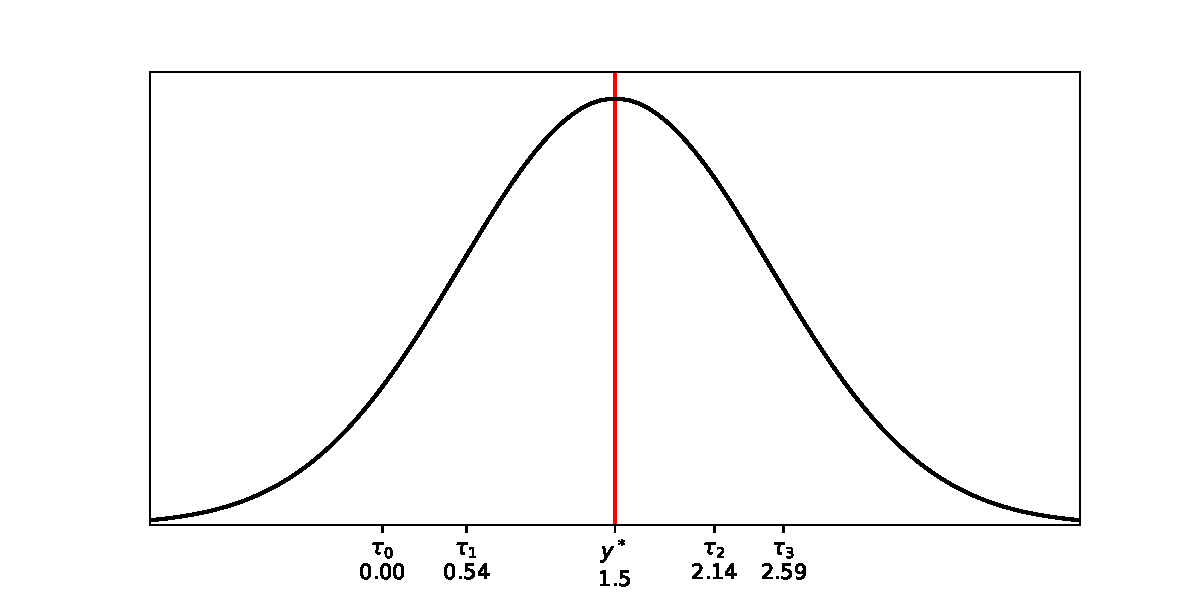
\includegraphics[width=\textwidth]{fig/oprobit_norm.pdf}}
  \only<3>{\centering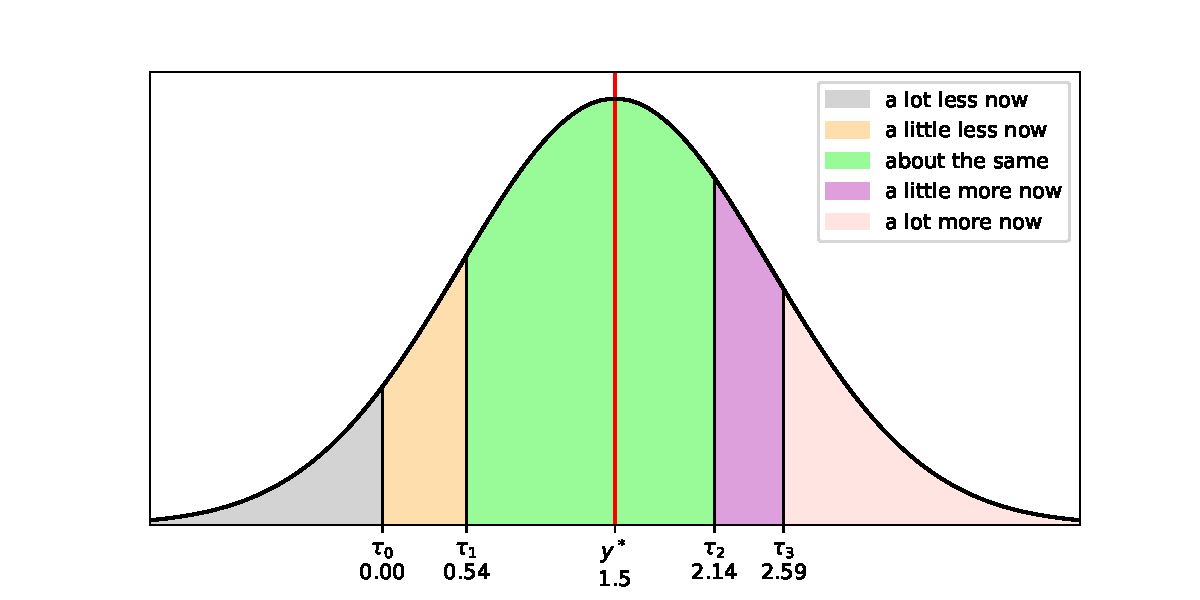
\includegraphics[width=\textwidth]{fig/oprobit_fill.pdf}}
  \only<4>{\centering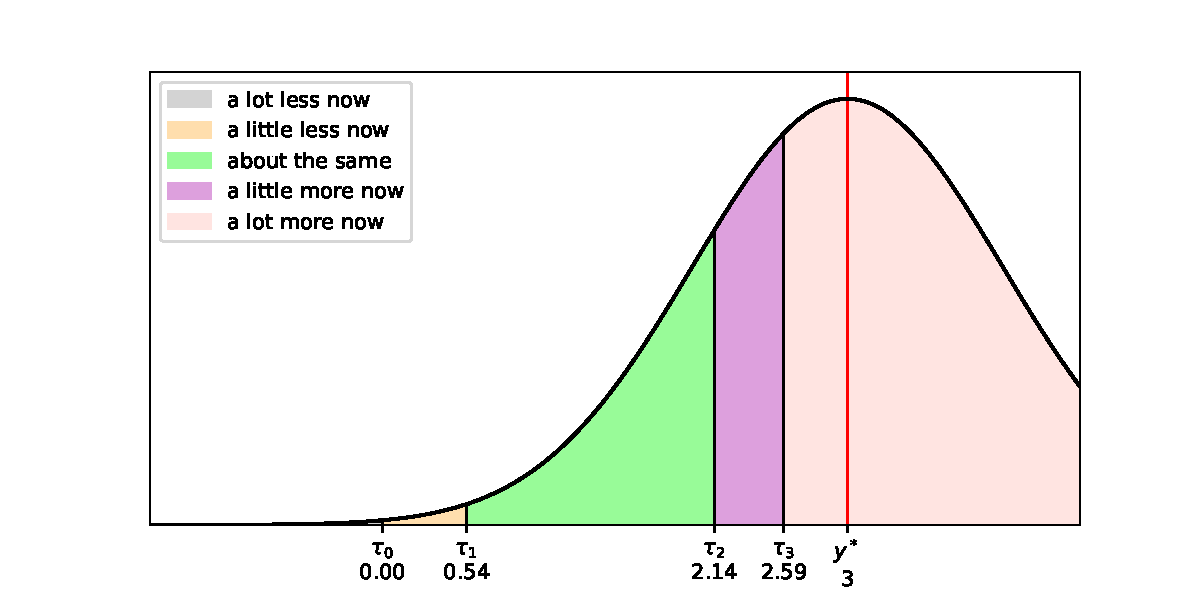
\includegraphics[width=\textwidth]{fig/oprobit_moved.pdf}}
  \\
  {\tiny Based on \textcite{handy_correlation_2005}}
\end{frame}
